\documentclass[10pt,a4paper]{article}
\usepackage[utf8]{inputenc}
\usepackage{amsmath}
\usepackage{amsfonts}
\usepackage{amssymb}
\usepackage{geometry}
\usepackage{verbatim}
\usepackage{enumerate}
\usepackage{fancyvrb}
\usepackage{graphicx}
\usepackage{tikz}
\usetikzlibrary{positioning}
\usetikzlibrary{shapes,snakes}
\usepackage[english]{babel}

\geometry{legalpaper, margin=1.5in}

\author{William Schultz}
\begin{document}
\title{Business and Finance}
\author{William Schultz}
\maketitle
 

All businesses should produce some amount of \textit{revenue}: the total amount of income generated by the sale of goods and services related to the primary operations of the business.
Revenue taken in is like a big pool of cash that the company can do things with. One key part is paying for the \textit{cost of goods sold} (COGS): the direct costs associated with producing the goods and services sold. For example, if you run a lemonade stand, what is the cost of the lemons, sugars, cups, etc. that you need in order to sell your product. Or, if you are a database company, this might include the cost to run servers or the underlying infrastructure that supports your service. This is money you must pay in order to function and sell a product.

\subsection*{Gross Margin}

A core related concept is \textit{gross margin}: the difference between total revenue and the cost of goods sold. If you take in \$100 in revenue and your COGS is \$10, then your gross margin is \$90. Typically, it makes sense to present this proportionally, as a percentage of revenue. That is,
\begin{align}
    \text{Gross Margin} = \dfrac{Revenue - COGS}{Revenue} \times 100
\end{align}

Money left over after paying for COGS is called \textit{gross profit}. This is then used to go ahead and pay for other expenses, like labor, sales/marketing, etc.

If you then take the \textit{gross profit} and deduct these other expenses, like R\&D, sales/marking, etc. then this gives you the \textit{operating margin} i.e telling you how much is left over after cost of goods sold and cost to basically run the business.
\begin{align}
    \text{Operating Margin} = \dfrac{Gross Profit - Operating Expenses}{Revenue} \times 100
\end{align}

\begin{figure}[h]
    \centering
    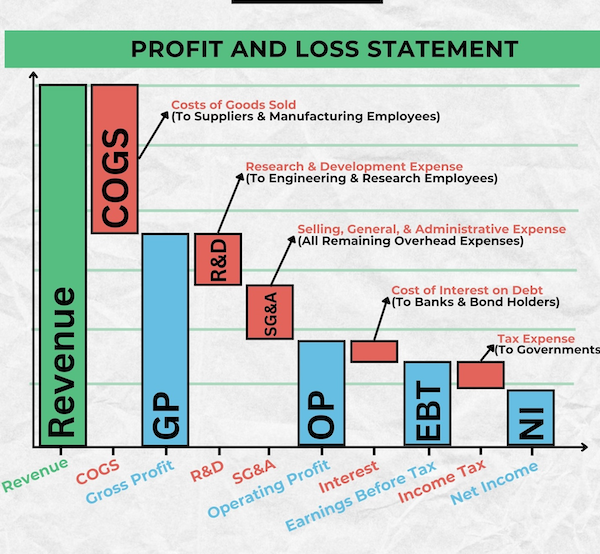
\includegraphics[width=0.55\textwidth]{images/pandl_visual.png}
    \caption{Gross margin and operating margin illustrated as an overall profit and loss statement.}
    \label{fig:gross_margin}
\end{figure}



\bibliographystyle{plain}
\bibliography{../../references.bib}

\end{document}